Outre son engagement fort en faveur de l’usage des technologies du web, \pense se distingue aussi d’un certain nombre de projets en humanités numériques français par son adoption explicite du \textit{design thinking}\footnote{Adoption revendiquée dans la présentation officielle du projet et réaffirmée dans le point d’étape suivant : \footcite{carius_plateforme_2020}} selon une impulsion donnée par l’ingénieur en charge du développement du projet. Ce cadre de réflexion, initialement formalisé dans le monde de l’industrie, est ancré dans un héritage méthodologique valorisant fortement les dimensions de créativité, de collaboration et de prise en compte du besoin de l’utilisateur dans la production de services ou de produits ; des perspectives entrant en résonnance avec un certain nombre d’approches, de pratiques voire de disciplines maintenant bien installées dans le monde large du développement logiciel et importées progressivement, par capillarité ou mimétisme, dans le monde de la recherche en humanités numériques, essentiellement dans la sphère anglo-saxonne. Nous étudierons dans ce chapitre les enjeux d’intégration de ce concept issu dans l’industrie dans le domaine des humanités numériques, tout particulièrement en histoire de l’art, puis nous nous pencherons sur une application concrète de cette méthode dans le cadre du développement de \pense. 

\subsection{Le \textit{design thinking} et son adoption dans les humanités numériques}

\subsubsection{Un concept venu du monde industriel, destiné à « stimuler l’innovation »}

Le  \textit{design thinking}, traduit en français sous le terme « pensée design », dont les contours et les interprétations sont parfois jugés flous\footcite[p.2]{kelly_design_2021}, est l’héritier d’une riche réflexion théorique développée dans le monde du design industriel dès les années 1950\footnote{Voir à ce propos l’ouvrage de Herbert A. Simon, The Sciences of the Artificial, 1969 définissant une « science du design ».}, s’intéressant notamment aux liens entre créativité, collaboration, conception design et résolution de problèmes. Voisin d’autres approches comme le design de service ou le design centré utilisateur (UCD), il a été formalisé comme méthodologie de gestion de projet par Rolf Faste, professeur à l’Université de Stanford dans les années 1980, puis par David Kelley\footnote{Son entreprise précédente (de la fusion de laquelle est notamment issu IDEO) avait participé au design de l’Apple Macintosh (1984), premier micro-ordinateur commercialisé doté d’une interface graphique (cité dans \footcite{vial_quappelle-t-_2012})}, co-fondateur de la firme de design IDEO (1991), avant d’être popularisé massivement par Tim Brown\footnote{Voir l’ouvrage de Tim Brown, Change by design : how design thinking transforms organizations and inspires innovation, 2009} (2008), PDG de cette même entreprise jusqu’en 2019. Nous nous référerons dans ce chapitre à l’acception du terme tel que défini par ce dernier, qui en a notamment simplifié certains principes, cette acception constituant l’approche retenue par l’ingénieur en charge du projet \pense. 

Lui octroyant une généalogie prestigieuse (au moins du point de vue américain) en la personne d’Edison, Brown décrit le \textit{design thinking} comme une véritable « discipline utilisant la sensibilité et les méthodes du designer pour satisfaire les besoins [des clients] avec [un projet] techniquement faisable et [économiquement] viable » \footcite[p.2]{brown_design_2008}. Il s’agit d’adopter une approche « empathique », ouverte d’esprit et volontiers créative (la dimension du « designer » s’inscrit aussi dans cette ambition) pour répondre à des besoins parfois exprimés de manière implicite ou naïve par un non-spécialiste. Les principes fondamentaux de la pensée design selon Tim Brown, qui synthétise ainsi les 7 étapes initialement développées par Rolf Faste (définition, recherche, brainstorming, prototypage, sélection, implémentation, apprentissage) sont une trinité : inspiration,  idéation (ou conceptualisation), implémentation. Le tout centré sur l’écoute et l’observation de l’utilisateur, la collaboration active entre professionnels de différentes disciplines et la production itérative de prototypes systématiquement soumis à la validation par l’utilisateur (ou à défaut, un échantillon représentatif de ce dernier). 

L’approche \textit{design thinking} rappelle beaucoup dans sa philosophie celle du design dit \ux, formalisée en 1988 par l’ouvrage de Donald Norman, \textit{The Design of everyday things}, avec qui elle partage le caractère « centré sur l’utilisateur » \footcite[p.175]{pelissier_accompagner_2017} et une partie de son héritage théorique. La différence la plus fréquemment relevée par les professionnels de l’« ergonomie digitale » est celle de la spécificité. Ainsi, quand le \textit{user experience design} se concentre véritablement sur la relation homme-machine et plus précisément, la conception d’interfaces utilisateur répondant à des besoins et des désirs précis, de manière à assurer une expérience la plus agréable possible pour l’utilisateur, le \textit{Design Thinking}, à la méthodologie volontairement pensée pour s’étendre à des domaines professionnels variés, qui dépassent le cadre du développement logiciel et d’interface, se conçoit plus largement comme un état d’esprit, une approche pouvant englober d’autres pratiques, dont l’UX. 

Cette approche partage un certain nombre de points communs avec les pratiques Agiles, popularisées par le \textit{Manifeste pour le développement Agile de logiciels}\footcite{noauthor_manifeste_nodate} (2001), qui prônent elles aussi des cycles de production « itératifs et incrémentaux », à l’opposé de l’approche « traditionnelle » des cycles de développement dits « en cascade » et des cycles « en V », adoptant plutôt une logique linéaire et séquentielle, pratiques issus du monde de l’industrie traditionnelle. 
Similairement au \textit{data storytelling} que nous évoquions plus tôt, bien le \textit{design thinking} soit souvent présenté comme une solution novatrice, ses principes sous-jacents sont bien antérieurs. En effet, l’ingénierie des facteurs humains (IFH), qui met en avant une prise en compte systématique des utilisateurs dès les phases initiales d'un projet, constitue un précédent notable. Cette discipline, qui s'intéresse à l'interaction entre les êtres humains et les systèmes, remonte à des décennies et s'est progressivement imposée dans de nombreux secteurs professionnels\footcite{vautier_ingenierie_1999}. 
Par ailleurs, le \textit{design thinking} est parfois accusé de manquer de contextualisation dans l’analyse des problèmes qu’il vise à résoudre. Ce manque de prise en compte des facteurs structurels, tels que les inégalités sociales ou économiques à l’origine des problèmes étudiés, a été décrit comme conduisant parfois à des recommandations peu réalistes, trop éloignées des réalités systémiques\footcite{ackermann_design_2023}. De plus, le processus tend à accorder une place prédominante aux designers, au détriment d’autres facteurs, notamment ceux liés à la spécificité des métiers concernés, ce qui peut engendrer une certaine déconnexion avec les enjeux propres à ces domaines.

\subsubsection{Vers une intégration dans les humanités numériques ?}

L'un des principaux arguments en faveur de l'intégration du \textit{design thinking} dans les humanités numériques réside dans la complémentarité de cette méthode avec les processus de recherche. En effet, la logique itérative du \textit{Design Thinking}, souvent fondée sur des cycles successifs de tests et de corrections, est susceptible, à notre sens, de s’accorder avec la démarche heuristique caractéristique de l’élaboration de la connaissance en sciences humaines. Dans le cadre du projet \pense, cette méthode itérative permet une expérimentation continue, encourageant l'essai et l'erreur (\textit{trial and error}) dans le développement de solutions numériques à destination du chercheur.
Le \textit{design thinking} s’intègre également assez naturellement dans les pratiques de management de projet au sein des humanités numériques. Il entend favoriser la diversification des équipes et le dialogue interdisciplinaire\footcite{peche_design_2016}, entrant ici en écho avec les principes mis en avant par les rédacteurs du \textit{Manifeste des Humanités Numériques}\footcite{dacos_manifeste_2011}. Comme le souligne \citeauthor{vial_tournant_2016}, le \textit{design thinking} permet de dépasser la simple commande technique d’un livrable pour adopter une démarche de « co-design », où les chercheurs collaborent dès les premières étapes de conception avec les « designers » et où les tâches de développement informatique et d’élaboration scientifique ne sont pas isolées l’une de l’autre\footcite{vial_tournant_2016}.
Un exemple, toujours cité par Stéphane Vial, illustrant cette approche est le projet \textit{VÉgA}, au cours duquel des égyptologues ont travaillé en étroite collaboration avec des designers pour « co-créer » les premiers « story-boards d'interaction » d’un projet d’interface. Ce processus a permis de repenser non seulement l’interface, mais aussi la manière d’interagir avec l’information, redéfinissant ainsi la relation entre le projet de recherche et son support numérique. Ce type de collaboration montre bien comment le \textit{design thinking} peut servir de médiateur entre les humanités numériques et les sciences de l’information, permettant une meilleure compréhension et manipulation des données\footcite{vial_tournant_2016}.
En outre, Anne Burdick et al., cités par Stéphane Vial, soulignent que les humanités numériques elles-mêmes en tant que discipline (ou « transdiscipline »), reposent en grande partie sur des cycles rapides de prototypage et de test, rappelant fortement ceux chers au \textit{Design Thinking}\footnote{\footcite{burdick_digital_humanities_2012} cité dans \footcite{vial_tournant_2016}}. Cette approche offre une flexibilité qui permet aux chercheurs d'ajuster en permanence leurs méthodes en fonction des retours d'expérience, un atout considérable dans un domaine où l'expérimentation et l’innovation sont centrales.

\subsubsection{Le \textit{design thinking} comme « cheval de Troie » néolibéral ? Une brève réflexion politique}

L’intégration du \textit{design thinking} dans les humanités numériques ne se fait pas sans soulever des préoccupations d’ordre polémique. Son origine commerciale et son association avec le monde de l’entreprise peut expliquer une possible réticence de la part de certains chercheurs en humanités à adopter les principes du \textit{Design Thinking}, y voyant un déplacement des valeurs académiques traditionnelles vers une approche plus orientée vers le marché et l'innovation commerciale\footcite[p.147-48]{grumbach_design_2023}. Il est possible de relier cette critique à une lecture de l’importation de pratiques jugées originellement « étrangères » aux humanités comme source de bouleversements non seulement épistémologiques mais politiques. 
Certains chercheurs sont ainsi susceptibles un processus d’importation de concepts propres au monde de l’entreprise, qui modifie profondément la manière dont les projets de recherche sont conçus et menés. L’introduction du « mode projet », délimité dans le temps, avec des objectifs précis et des enjeux de production de résultats peut être rapprochée de la réflexion de \citeauthor{pawlicka_data_2017} au sujet de la scientifisation des humanités\footcite{pawlicka_data_2017}. Cette approche contraste avec la nature de la recherche académique, davantage centrée sur le processus que sur l’aboutissement d’un produit fini.
L’adoption du \textit{design thinking} dans les humanités numériques peut ainsi être perçue comme une tentative de faire de ces disciplines un champ « pratique, innovant et profitable », une tendance qui est encouragée par des impératifs économiques similaires à ceux qui régissent les entreprises\footcite[p.526-28]{pawlicka_data_2017}. L'importation de concepts issus du monde entrepreneurial n'est pas un choix neutre, surtout lorsque le \textit{design thinking} lui-même est présenté comme une « approche managériale de l'innovation » \footcite[p.12]{peche_design_2016}. Cette logique trouve écho chez une lecture interrogeant le mode projet, cher au \textit{Design Thinking}, comme un possible « cheval de Troie » néolibéral, infiltrant progressivement les humanités à travers leur composante numérique\footcite{smaniotto_dh_2014}.

\subsection{Chronologie d’une gestion de projet : développement d’un bouton de citation automatique de l’édition \textit{Barye}, selon les principes du \textit{design thinking}}

Un exemple concret de l'application des principes du \textit{design thinking} au sein du projet \pense est le développement d’un petit outil (sous forme de bouton cliquable de type « \textit{popover} » \footcite{otto_popovers_nodate}) permettant de citer automatiquement en un clic et selon un format de citation bibliographique établi auprès du chercheur ayant émis le besoin, chaque page de l’édition numérique des \textit{Papiers Barye}. Il a été réalisé en collaboration avec l’ingénieur en charge du projet, et en suivant les principes du \textit{design thinking} tels qu’assimilés au sein de \pense. Cet outil est accessible pour chaque document disponible (sous sa version améliorée par l’ingénieur en charge du projet) sur l’édition numérique, en suivant le modèle suivant : https://barye.inha.fr/document/[cote\_identifiant\_le\_document]/?mode=citation. 

\begin{figure}[h] 
\centering 
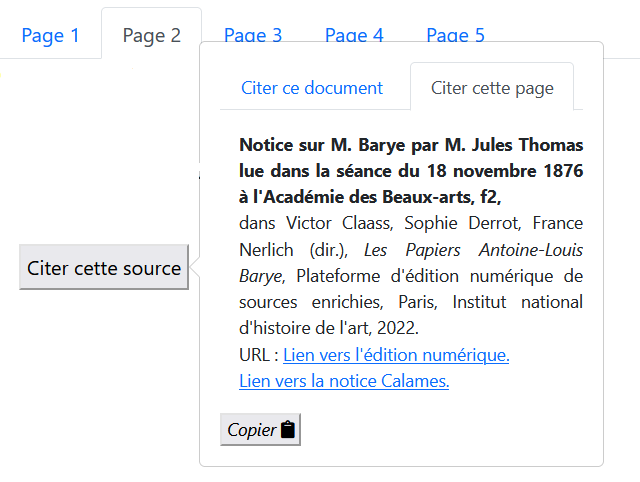
\includegraphics[width=0.8\textwidth]{bouton_citation_transfo_citation_indiv} 
\caption{Prototype de bouton de citation (page de test) tel que produit à l’issue de trois semaines de processus itératifs dans le cadre du stage.} 
\label{fig:prototype-bouton} 
\end{figure}

Les étapes de conception de cet outil suivent les trois phases du \textit{design thinking} décrites par Brown : « inspiration », « idéation » et « implémentation » \footcite[p.5]{brown_design_2008}. Dans un premier temps, les besoins des utilisateurs ont été identifiés, puis conceptualisés sous forme de modélisations, avant d’être finalement implémentés dans une solution fonctionnelle prototypée ayant fait l’objet de plusieurs améliorations accueillant les suggestions émises par le chercheur à l’origine de la demande. 

\subsubsection{Prendre en compte les besoins de l’utilisateur (« empathie »)}

La première étape du processus de \textit{design thinking} consiste à recueillir des informations précises en dialogue avec l’utilisateur final, ici représenté en la personne du chercheur, pour mieux comprendre ses besoins. Ce processus repose sur l’écoute attentive et sur une évaluation équilibrée entre le souhait exprimé par le client et les contraintes techniques ou de faisabilité qui peuvent en découler. Comme le souligne Tim Brown, cette approche est indispensable pour s’assurer que le résultat final correspond non seulement aux attentes, mais qu’il soit également viable dans un contexte de mise en œuvre réelle\footcite{brown_design_2008}.
Dans le cadre du projet \pense, la collecte des informations s’est effectuée sous la forme d’une série de réunions, notamment une réunion initiale, au cours de laquelle le chercheur a pu formuler ses demandes. Une demande spécifique a émergé concernant l’ajout d’un bouton sous forme de pop-over, évoqué plus haut. Celui-ci devait contenir deux onglets : un pour générer une citation l’échelle du document et l’autre à l’échelle de la page individuelle sélectionnée. De plus, un format précis de citation bibliographique a été requis afin de permettre aux utilisateurs de citer facilement les documents présents dans l’édition numérique.
\newline
\textbfit{Familiarité}\\

Comprendre l’usage que les chercheurs font de ces outils constitue une dimension essentielle du \textit{Design Thinking}. Il s’agissait ici de comparer les outils analogues existants sur d’autres plateformes familières aux chercheurs, telles qu’\textit{OpenEdition}, afin d’évaluer les bonnes pratiques en termes d’ergonomie et de proposer une solution facilement appropriable par l’utilisateur ciblé. Parmi les critères analysés figuraient l’intelligibilité de l’outil, sa praticabilité et son assimilation à des codes communs, comme celui du « clipboard », ou presse-papier. En exploitant cette familiarité, l’objectif est de s’assurer que l’utilisateur puisse naviguer aisément dans l’outil, sans avoir besoin de réfléchir excessivement à son fonctionnement – un principe cher au consultant UX Steve Krugs dans son ouvrage intitulé \textit{Don't Make Me Think }.
\newline
\textbfit{Intérêt scientifique de l’outil}\\

Un autre point fondamental à prendre en compte dans la conception de cet outil est son intérêt scientifique, et plus particulièrement la question de la citation. Rendre une édition numérique aisément « citable » est un facteur essentiel pour la diffusion et la reconnaissance scientifique de cette dernière\footcite{sahle_what_2016}. En effet, l’acte de citation permet non seulement de certifier la légitimité d’un document scientifique, mais aussi de favoriser sa réutilisation par la communauté académique, contribuant ainsi à la circulation du savoir. Il s’agit donc de faciliter au maximum l’intégration de l’édition numérique dans le paysage des productions en humanités numériques – un enjeu de taille.
\newline
\textbfit{Réunions régulières pour affiner le projet}\\

Le processus de création de cet outil s’est déroulé de manière itérative, avec des réunions régulières organisées entre les chercheurs, les concepteurs et les ingénieurs. Cette démarche rappelle les méthodes de « co-conception centrée-utilisateur » observées dans d’autres projets comme \textit{Vega}, où les réunions permettent d’ajuster continuellement le prototype afin de mieux répondre aux attentes des utilisateurs\footcite{vial_tournant_2016}. Des réunions effectuées le 15 avril, le 21 et le 29 mai ont été effectuées afin de corriger les prototypes présentés et garantir leur bonne correspondance aux attentes de la recherche.
Parmi les réunions-clés, celle du 15 avril fut dédiée à l’ajustement des aspects formels, tels que l’italique, la longueur des citations, le format de déploiement des URL, l’intégration de liens externes pointant vers les ressources archivistiques (\textit{Calames}) et l’usage d’une virgule plutôt que par des parenthèses pour la séparation de l’URL avec le reste de la citation. Ces ajustements sont essentiels pour s’assurer que les utilisateurs puissent intégrer les citations sans devoir effectuer des corrections manuelles par la suite, garantissant ainsi une cohérence entre les exigences scientifiques et l’ergonomie de l’outil.
Le 21 mai, en préparation de la réunion de pilotage, d’autres éléments formels ont été discutés, notamment la dimension design (volonté d’encadrer les citations) et la nécessité d’adapter les boutons de citation aux parcours spécifiques de l’édition \textit{Barye}, étendant donc l’usage de l’outil au-delà de l’édition des documents manuscrits, en l’intégrant aux commentaires critiques. Une réflexion linguistique a également été menée sur l’usage ou non de l’article démonstratif (« Citer \textit{ce} document » contre « Citer \textit{le} document ») et son impact sur la bonne ergonomie de l’outil. 
\newline
\textbfit{Apport de l’interdisciplinarité}\\

Le processus de conception ne se limitait pas à une approche technique, mais impliquait également une réflexion interdisciplinaire. La réunion du comité de pilotage de \pense du 29 mai illustre cette dimension, en réunissant des experts issus des domaines de l’archivistique, de la bibliothéconomie et des sciences humaines, permettant d’apporter un regard extérieur bienvenu sur la mise en œuvre de l’outil. Ces discussions ont permis d’aborder des questions terminologiques, comme l’usage des termes « feuillet », « page » ou « vue » pour désigner les possibles subdivisions présentes à l’échelle du document, qui selon la matérialité des documents cités et le point de vue adopté sur l’édition, peuvent s’avérer impropres sur le plan archivistique. 

\subsubsection{Modéliser les fonctionnalités attendues (« conceptualisation »)}

Une fois les besoins de l’utilisateur clairement identifiés, la modélisation des fonctionnalités attendues constitue l’étape suivante du processus de conception. Cette phase permet notamment de s’assurer que les parties prenantes – chercheurs, ingénieurs et autres collaborateurs – partagent une vision commune du projet. L’esquisse de storyboards rudimentaires permet ainsi de représenter graphiquement les idées, et vise à dissiper d’éventuelles incompréhensions susceptibles d’émerger à partir des échanges oraux ou des instructions écrites. Ces storyboards, inspirés de l’industrie cinématographique, servent de support visuel aussi bien aux collaborateurs techniques qu’au « client », ici, le chercheur. Une modélisation rudimentaire permet ainsi de vérifier que toutes les parties prenantes sont alignées sur les mêmes objectifs, tout en mobilisant des ressources moindres qu’un véritable prototype.

\subsubsection{Créer, tester et affiner (« prototypage »)}\footnote{« iterative cycles of prototyping, testing and refinement » in \footcite[p.4]{brown_design_2008}}

Le processus de développement d’un projet numérique tel que \pense suit une approche caractérisée par des cycles itératifs de création, de test et d’affinement progressif, en cohérence avec les principes du \textit{Design Thinking}. 
Les réorientations successives du projet illustrent cette dynamique. Dans une première phase, une solution entièrement implémentée en JavaScript avait été ainsi envisagée, motivée par la grande flexibilité permise par ce langage. Celle-ci avait pour objectif d’intégrer dynamiquement des feuilles de style XSLT (permettant l’extraction des données textuelles de la base de données \tei et leur transformation en \html « exposable » sur le Web) au JavaScript à travers des requêtes AJAX. Toutefois, cette proposition n’a pas été retenue, ayant été jugée trop complexe et peu adaptée à l’architecture technologique préconisée par l’ingénieur en charge du projet, dans laquelle l’intervention de JavaScript doit se situer en aval, c’est-à-dire au moment du chargement de la page dans le navigateur, et non dans l’interaction avec le serveur (traduisant une approche plus traditionnelle dans l’usage de ce langage). Tandis que des technologies comme XSLT sont davantage employées côté serveur, en amont, pour transformer des données structurées, telles que des documents \xml, avant leur affichage dans le navigateur. Cette séparation des rôles technologiques a donc conduit à une révision de la stratégie initiale adoptée pour le projet \pense. 
\newline
\textbfit{Scripts élaborés}\\

Plusieurs scripts ont été élaborés, essentiellement en XQuery et Python. Les scénarios de transformation XSLT/XQuery visaient à extraire, en temps réel, les informations nécessaires depuis la base de données et à les intégrer sous forme de citations prêtes à l'emploi. Deux approches ont été explorées dans ce cadre : d'une part, la transformation de données en \html accompagnée de code JavaScript, et d'autre part, leur intégration dans des modèles \html préexistants.
Les scripts développés pour la gestion du bouton de citation étaient conçus pour répondre aux besoins spécifiques du projet tout en tenant compte des contraintes techniques imposées par le format des données sources. Les langages utilisés, XQuery et XSLT, se sont révélés adaptés pour manipuler des documents \xml complexes.

Dans le cadre du traitement des fichiers \xml au format \tei, plusieurs scripts intermédiaires ont dû être créés pour répondre à des besoins spécifiques de pré-traitement et d'alignement des données. L’un des premiers scripts développés visait à corriger un problème récurrent dans les fichiers \tei : la présence d’espaces insécables. Ces caractères invisibles provoquaient des erreurs dans le traitement automatique des données. Pour y remédier, un script en Python a été créé pour automatiser leur suppression, normalisant ainsi les fichiers avant leur traitement ultérieur.
Un autre défi technique important a été l’alignement des identifiants entre deux documents \xml distincts et de grammaire différente (\tei et \ead), afin de permettre une mise en concordance des identifiants adossés aux fichiers de la base de données \xml-\tei de \pense avec les identifiants des archives matérielles correspondantes de la base Calames (dont la description est structurée en \xml-\ead, standard pour l’encodage d’inventaires archivistiques). Calames, le \textit{Catalogue en ligne des archives et manuscrits de l’enseignement supérieur}, utilise un système de cote différent de celui adopté en interne par \pense. La principale difficulté résidait dans la différence de granularité entre les identifiants \ead et \tei (les identifiants \tei étant plus précis que les identifiants \ead). Cependant, les deux types de documents partageant une structure arborescente commune, fondée sur le \xml, il a été possible d'utiliser des outils comme XQuery et des bibliothèques Python (telles que \textit{lxml} et \textit{ElementTree}) pour traiter cette correspondance.
Le script développé pour cette tâche avait pour objectif d’automatiser l’extraction des identifiants \tei et leur transformation afin de les aligner avec les identifiants \ead. Le processus débute par l'extraction des identifiants \tei depuis les fichiers correspondants grâce à la bibliothèque \textit{lxml}. Une fois extraits, ces identifiants sont ensuite transformés pour correspondre au format des identifiants \ead. Cette transformation se fait principalement par la normalisation des chaînes de caractères, en supprimant les zéros initiaux et en reformulant la structure des identifiants afin qu’ils soient plus compatibles avec les conventions de nommage du document \ead.
Le script permet ensuite de comparer les identifiants \tei normalisés avec les identifiants \ead, en effectuant une correspondance basée sur une comparaison caractère par caractère. Un algorithme de recherche du « meilleur match » est employé pour déterminer les correspondances les plus précises possibles entre les deux ensembles d’identifiants. Finalement, les résultats de cet alignement sont exportés dans un fichier \csv pour une exploitation future. Ce script constitue une étape importante dans l'enrichissement des métadonnées associées aux documents traités, facilitant ainsi l’intégration du bouton de citation.
\newline
\textbfit{Validation, visualisation et tests}\\

La phase de prototypage, en complément avec la modélisation conceptuelle, étant primordiale pour s’assurer que les solutions proposées répondent aux besoins des utilisateurs finaux, c’est dans cet esprit qu’ont été préparés deux documents destinés à une présentation devant le chercheur principal du projet le 15 avril. Ces documents avaient pour objectif de démontrer l’état d’avancement du prototype du bouton de citation, en particulier sur les aspects liés à l’affichage des données textuelles et à la visualisation des informations sous forme de « cartes ».
Bien que les codes produits à ce stade n’étaient pas conçus pour être des produits finis\footcite[p.3]{brown_design_2008}, ils permettaient d’avoir une vue d’ensemble du système en développement et de tester différentes configurations. Une visualisation par cartes utilisant le \textit{framework} \textit{Bootstrap} a notamment été proposée pour identifier rapidement les anomalies typographiques présentes dans les données textuelles extraites de la base et utilisées pour la citation ; ainsi que les éventuels problèmes dans l’affichage des citations.
Cette étape a permis d’affiner les choix de conception en fonction des retours du chercheur, confirmant ainsi l’adéquation entre les besoins du projet et les solutions technologiques mises en œuvre. De plus, cette démarche s’inscrit dans une logique itérative qui consiste à ajuster continuellement les solutions en fonction des retours des utilisateurs.
